
\documentclass[a4paper,11pt]{report}

%%%%%%%%%%%%%%%%%%%%%%%%%%%%%%%%%% Packages %%%%%%%%%%%%%%%%%%%%%%%%%%%%%%%%%%

\usepackage[utf8]{inputenc}
\usepackage{graphicx}
\usepackage[T1]{fontenc}
\usepackage[french]{babel}
\usepackage{float}
\usepackage{amsmath, amssymb}
\usepackage{geometry}
\usepackage{siunitx}
\geometry{margin=2.5cm}
\usepackage{hyperref}

\newcommand{\HRule}{\rule{\linewidth}{0.5mm}}

\begin{document}


%%%%%%%%%%%%%%%%%%%%%%%%%%%%%%%%%% Title Page %%%%%%%%%%%%%%%%%%%%%%%%%%%%%%%%%%

\begin{center}

% Upper part of the page. The '~' is needed because only works if a paragraph has started.
\includegraphics[width=0.55\textwidth]{Image/logo.png}~\\[1cm]

\textsc{\LARGE Telecom Physique Strasbourg}\\[1.5cm]

\textsc{\Large }\\[0.5cm]

% Title
\HRule \\[0.4cm]

{\huge Grating Coupler Fibre-Puce en Silicium \bfseries  \\[0.4cm] }

\HRule \\[1.5cm]

\begin{minipage}{0.4\textwidth}
\begin{flushleft} \large
\emph{Author:}\\
Nolan \textsc{LE TYRANT}\\

\end{flushleft}
\end{minipage}
\begin{minipage}{0.4\textwidth}
\end{minipage}

\vfill

% Bottom of the page
{\large \today}

\end{center}
\thispagestyle{empty}

\tableofcontents
%%%%%%%%%%%%%%%%%%%%%%%%%%%%%%%%%% Chapitre 1 : Introduction %%%%%%%%%%%%%%%%%%%%%%%%%%%%%%%%%%

\chapter{Introduction}

\section{Contexte et objectifs}

Les coupleurs à réseau sont des composants clés de la photonique intégrée sur silicium : ils permettent de coupler efficacement la lumière d'une fibre optique, arrivant en espace libre, vers le mode guidé d'un circuit photonique sur puce. Ce type de composant est par exemple utilisé pour l'interfaçage optique de circuits intégrés en photonique silicium.

L'objectif de ce projet est de concevoir, simuler et optimiser un coupleur à réseau fibre-puce en silicium, à l'aide de la méthode FDTD (Finite-Difference Time-Domain), et d'en maximiser l'efficacité de couplage à la longueur d'onde de 1{,}55~\textmu m (longueur d'onde télécom standard). Plus précisément, ce travail vise à :

\begin{itemize}
    \item établir une estimation analytique initiale de la géométrie du réseau, à partir de la condition d'accord de phase 
    \item mettre en œuvre une simulation FDTD du dispositif, avec une source représentant le mode d'une fibre optique monomode 
    \item valider numériquement la fiabilité des résultats obtenus, en identifiant et corrigeant les artefacts propres à la méthode FDTD 
    \item optimiser les paramètres géométriques du réseau (période, duty cycle) par balayage paramétrique, puis par une méthode d'optimisation par gradient 
    \item discuter des limites de l'approche et des pistes d'amélioration possibles
\end{itemize}

\section{Démarche générale}

La démarche suivie combine approche analytique et simulation numérique. Une première estimation de la période du réseau est obtenue analytiquement (chapitre~\ref{ch:theorie}), à partir d'un modèle simplifié de l'indice effectif du mode guidé. 

Les tout premiers résultats de simulation ayant révélé des incohérences dues à des artefacts de discrétisation spatiale, une étape de validation numérique (chapitre~\ref{ch:validation}) a été nécessaire avant de pouvoir interpréter les résultats d'optimisation. Cette validation comprend une étude de l'alignement spatiale entre la grille de calcul et le dispositif ainsi qu'une étude de convergence en résolution.

Une fois la méthode validée, les paramètres géométriques du réseau (période $\Lambda$ et duty cycle $gdc$) ont d'abord été manuellement optimisés par balayage paramétrique, puis par une méthode d'optimisation par gradient (chapitre~\ref{ch:resultats}).

\section{Plan du rapport}

Le chapitre~\ref{ch:theorie} présente le modèle théorique du couplage par réseau et l'estimation analytique initiale de la période. Le chapitre~\ref{ch:numerique} détaille la mise en œuvre de la simulation FDTD et les paramètres physiques retenus. Le chapitre~\ref{ch:validation} présente la démarche de validation numérique ayant permis d'établir la fiabilité des résultats. Le chapitre~\ref{ch:resultats} présente les résultats d'optimisation, obtenus par balayage manuel puis par méthode de gradient. Enfin, la conclusion revient sur les limites du travail réalisé et propose des pistes d'amélioration.

%%%%%%%%%%%%%%%%%%%%%%%%%%%%%%%%%% Chapitre 2: Théorie %%%%%%%%%%%%%%%%%%%%%%%%%%%%%%%%%%
\chapter{Modèle théorique}
\label{ch:theorie}

\section{Description du dispositif}
Le dispositif simulé est composé d'un faisceau incident (supposé arrivé par une fibre optique) avec un angle $\theta$ sur un réseau périodique de dents suivi d'un mode guidé. Le schéma du dispositif est le suivant:
\begin{figure}[h]
    \centering
    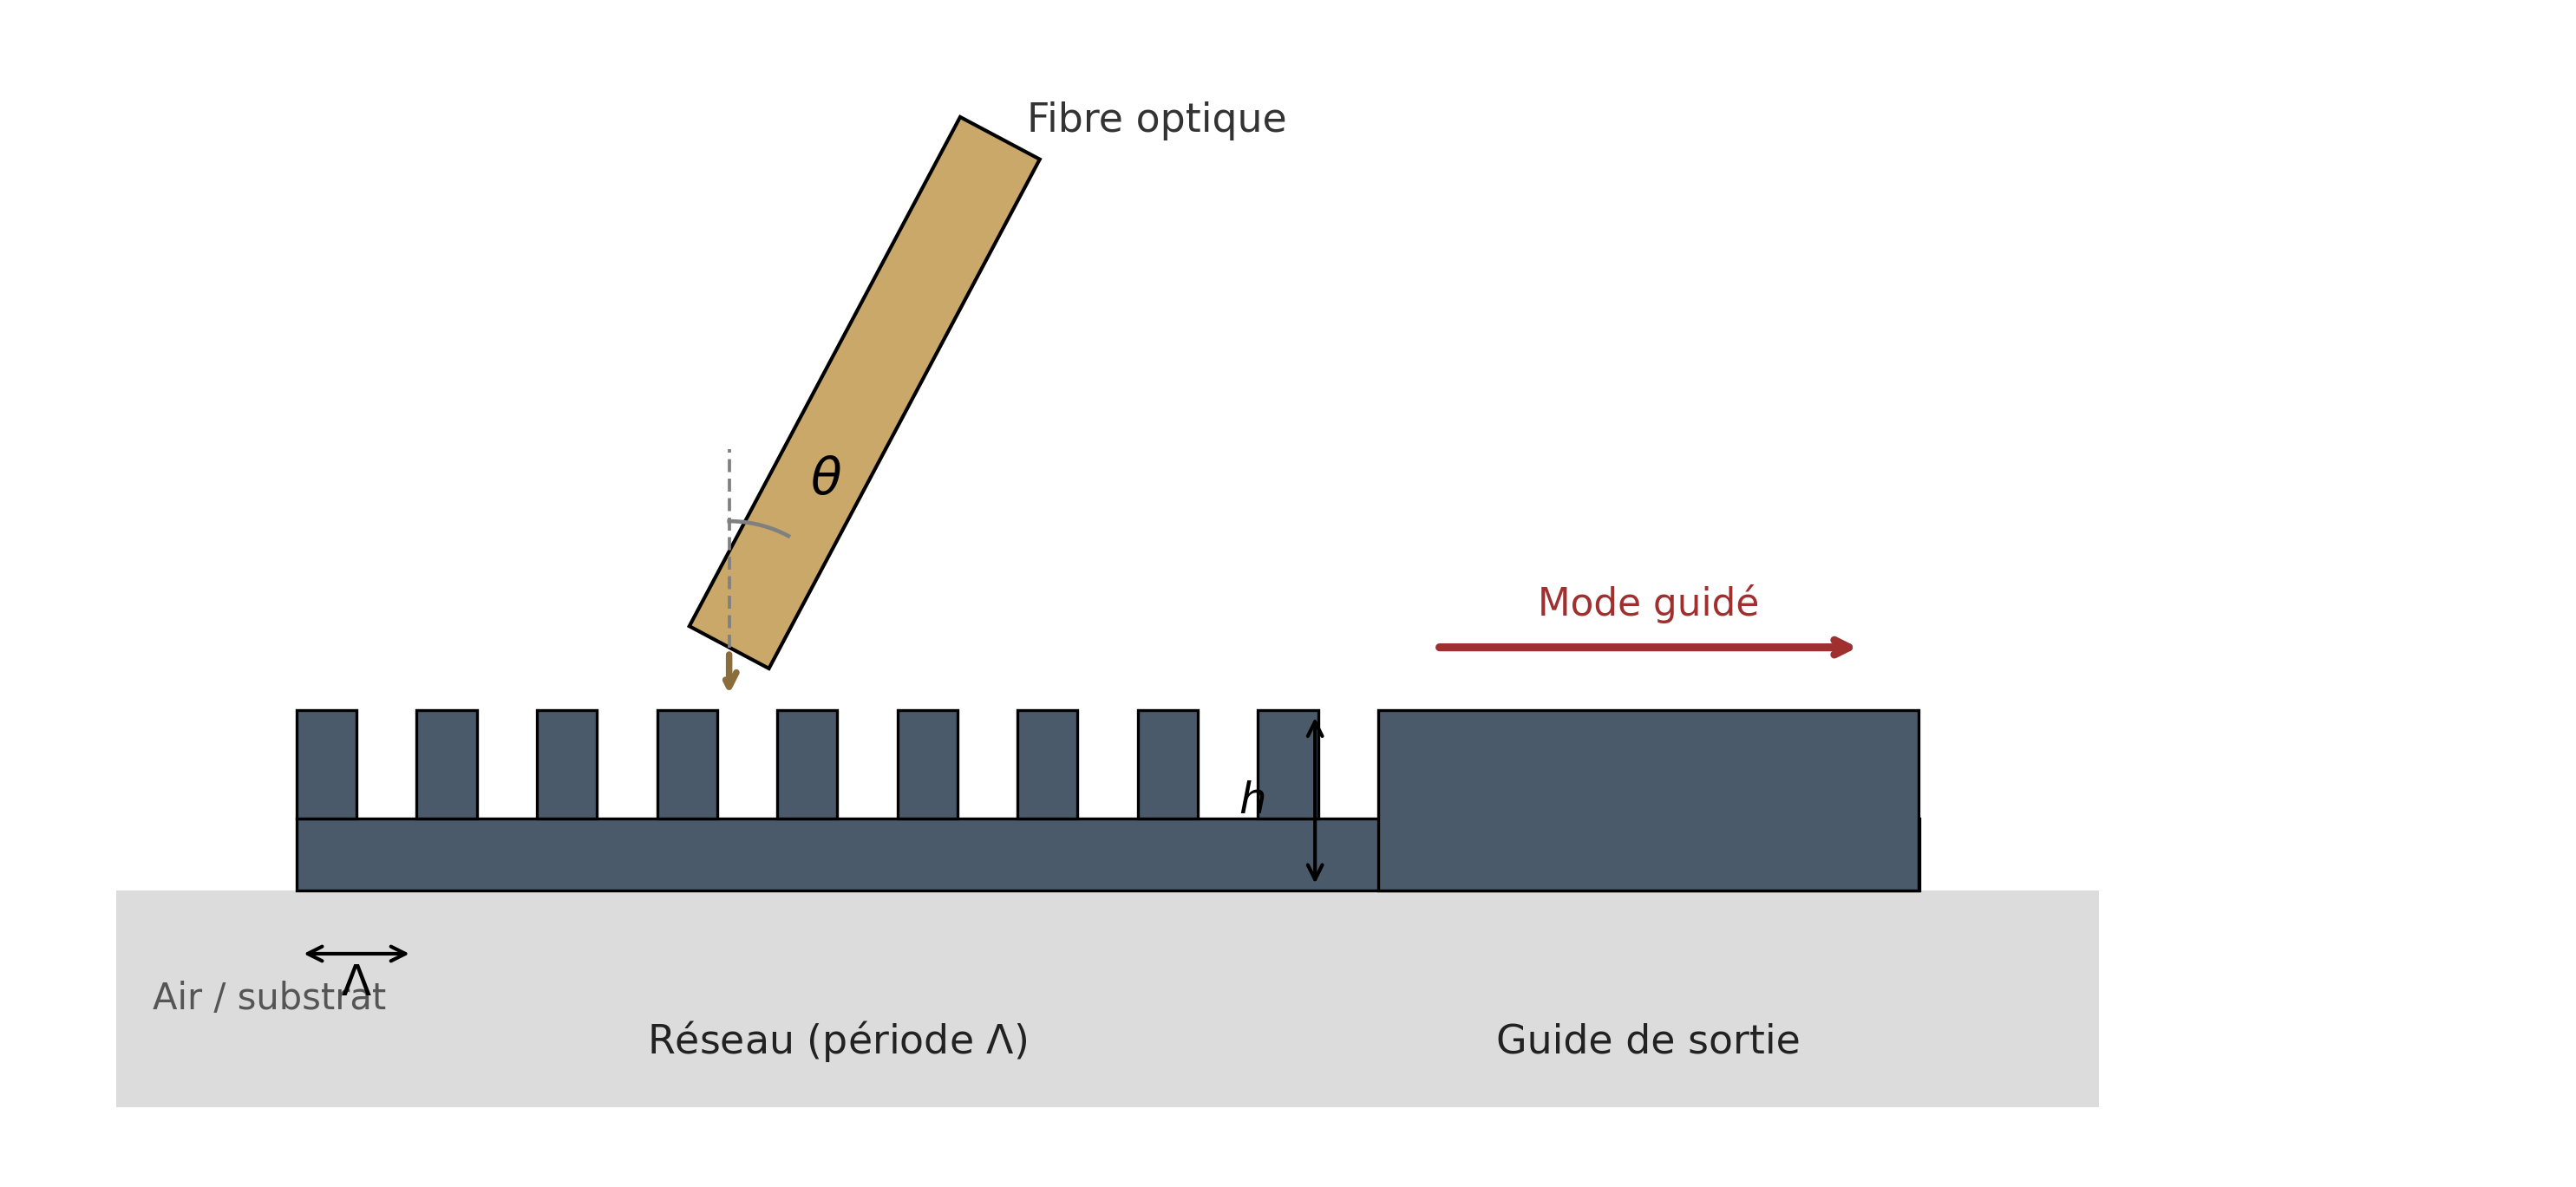
\includegraphics[width=0.85\linewidth]{Image/shema.png}
    \caption{Schéma du dispositif modélisé : fibre optique inclinée, réseau de diffraction, guide de sortie}
    \label{fig:schema_dispositif}
\end{figure}

\section{Condition d'accord de phase}

Le réseau doit rediriger la lumière incidente, arrivant en espace libre, vers le mode guidé du silicium. Cette condition se formule comme une condition d'interférence constructive entre les contributions successives des dents du réseau, analogue à la condition classique des franges brillantes en optique, où la différence de marche entre deux chemins doit être un multiple entier de la longueur d'onde.

\subsection*{Calcul des deux chemins optiques}

Considérons deux dents consécutives du réseau, séparées de la période $\Lambda$ (figure~\ref{fig:diff_marche}).

\begin{figure}[h]
    \centering
    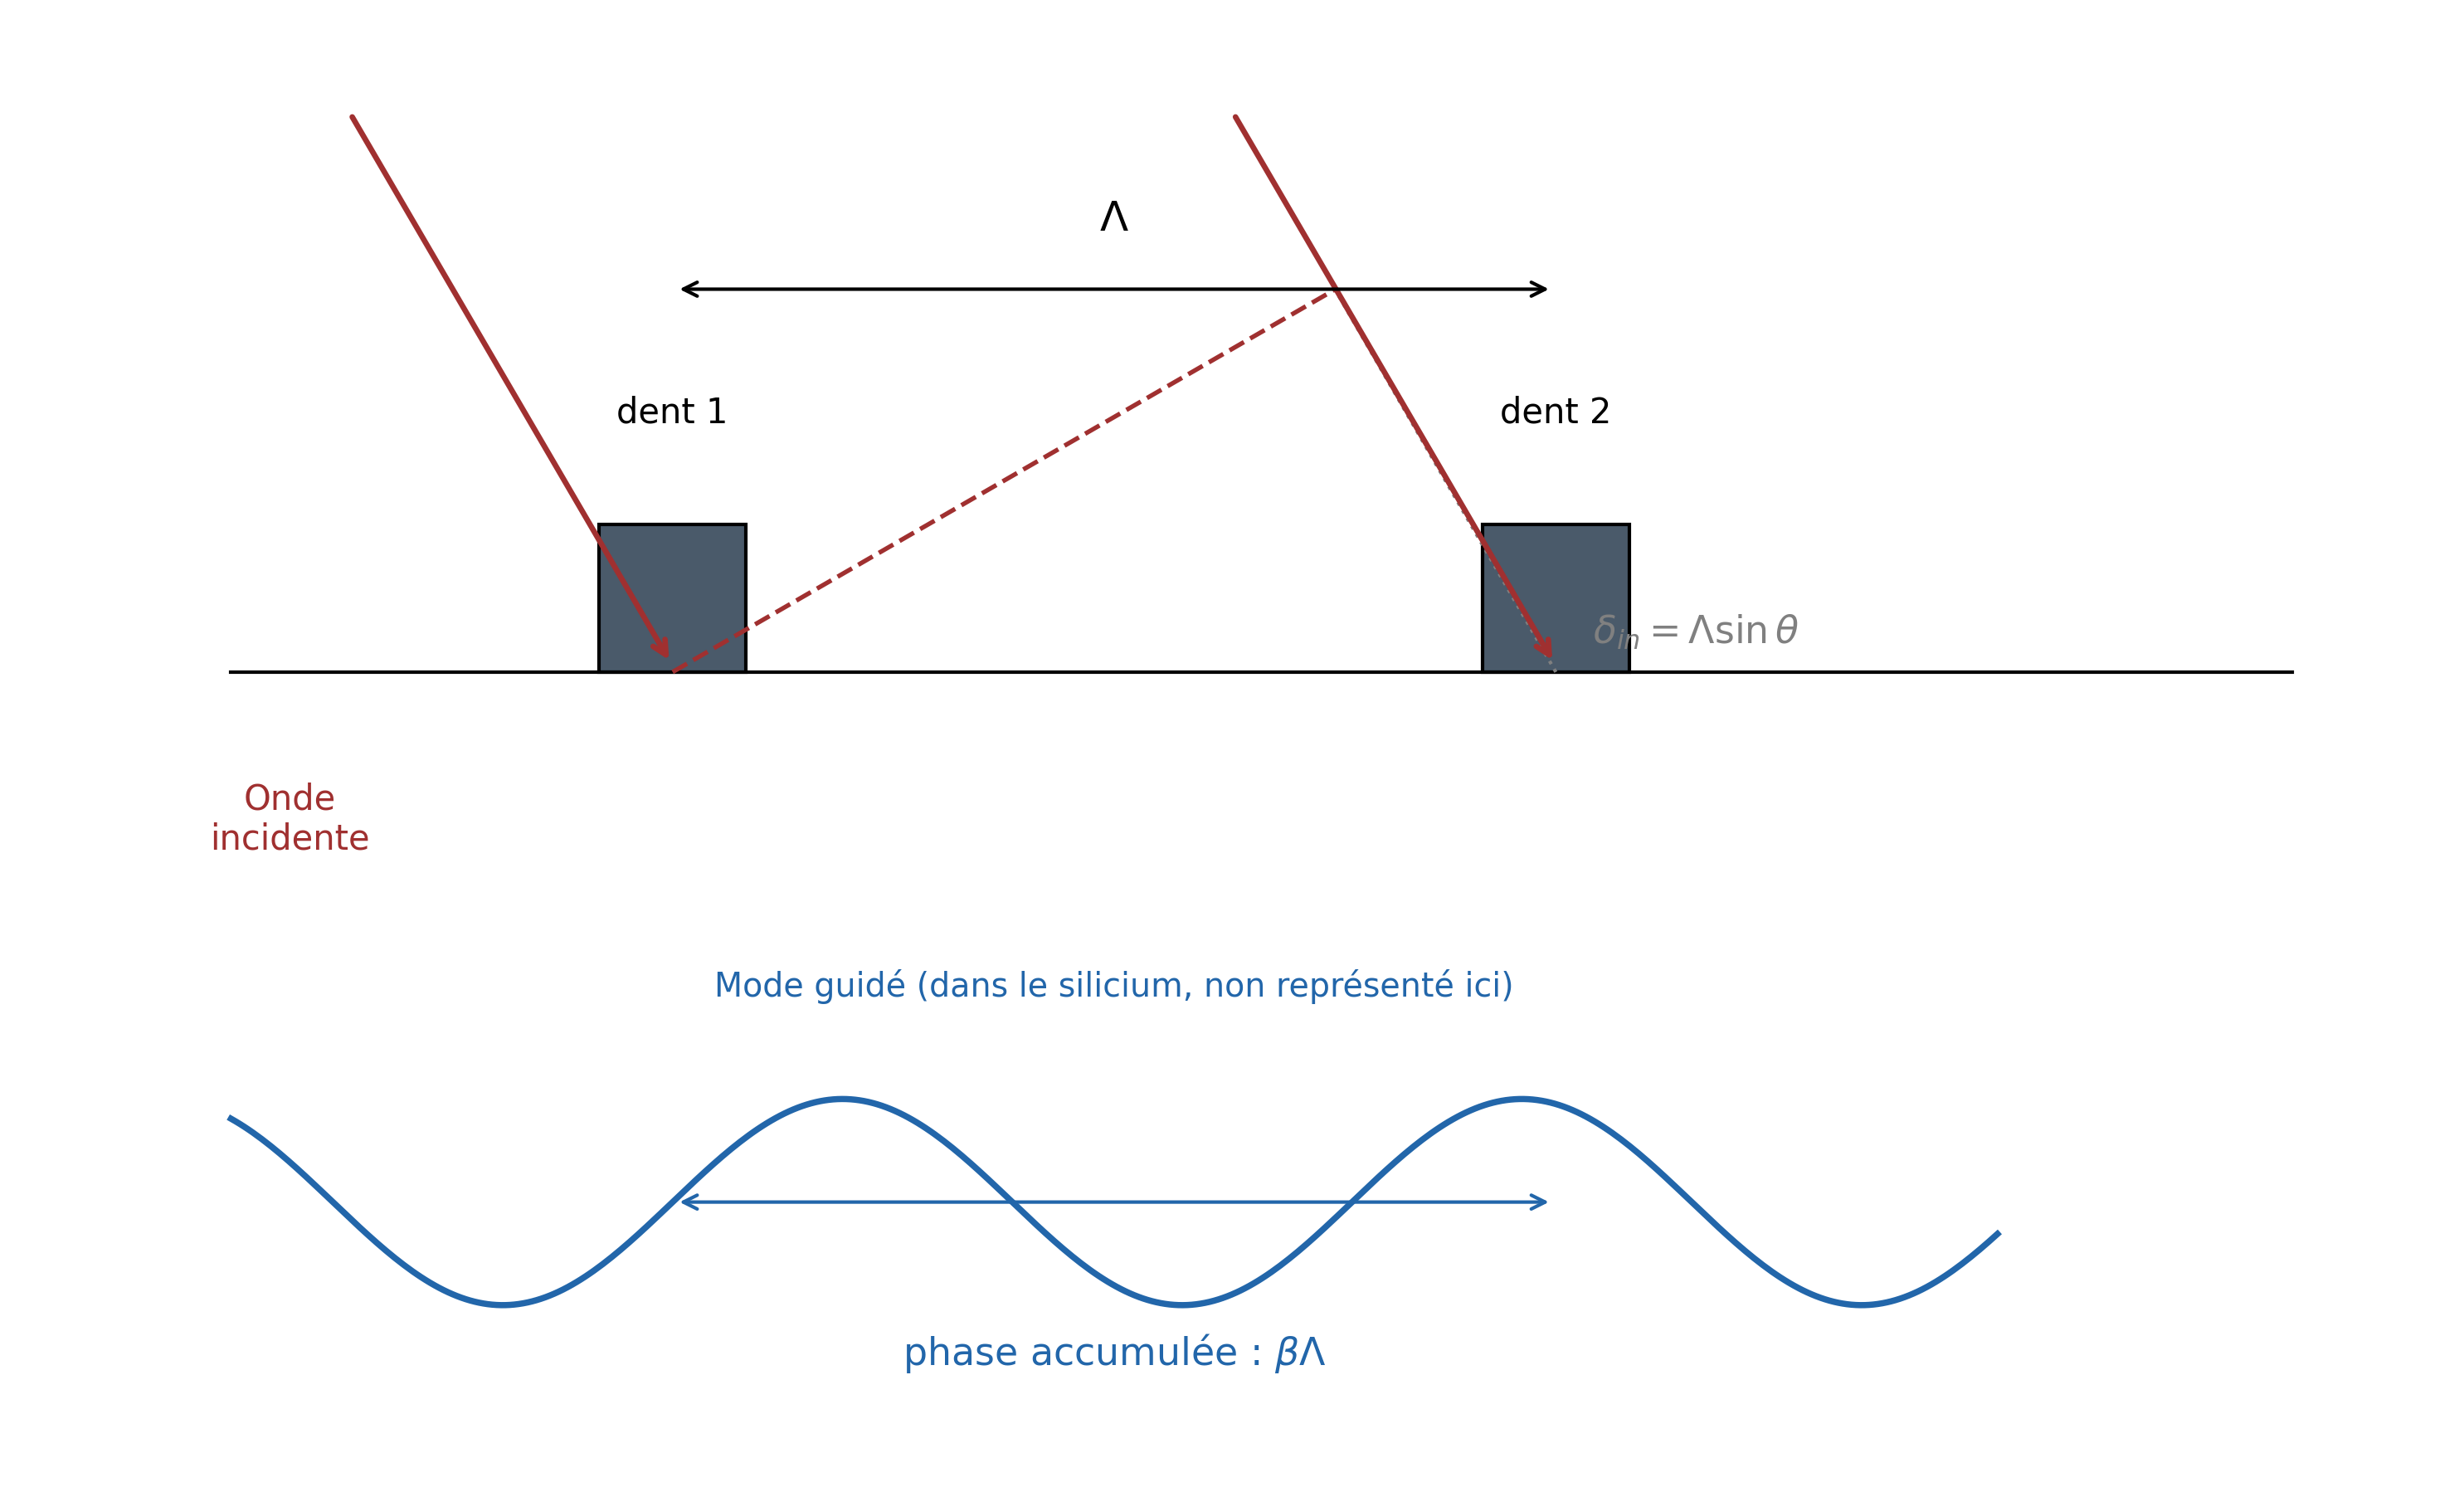
\includegraphics[width=0.85\linewidth]{Image/accord_de_phase.png}
    \caption{Différence de marche entre deux dents consécutives du réseau : $\delta_{in}$ côté onde incidente, $\delta_{guide}$ côté mode guidé}
    \label{fig:diff_marche}
\end{figure}

\paragraph{Chemin optique côté onde incidente.} L'onde incidente, arrivant avec un angle $\theta$ par rapport à la normale, atteint la seconde dent avec un retard géométrique par rapport à la première. Ce retard correspond à une distance de propagation supplémentaire dans le milieu incident (air, indice $n_{clad}$) :
\begin{equation}
\delta_{in} = n_{clad}\cdot\Lambda\sin\theta
\end{equation}

\paragraph{Chemin optique côté mode guidé.} Le mode guidé, une fois excité, se propage dans le guide avec un indice effectif $n_{eff}$ (calculé en section~\ref{sec:calcul_neff}). Le chemin optique qu'il parcourt sur cette même distance $\Lambda$ est :
\begin{equation}
\delta_{guide} = n_{eff}\cdot\Lambda
\end{equation}

\subsection*{Condition d'interférence constructive}

Pour que les contributions successives des dents s'additionnent de façon constructive dans le mode guidé, la différence de marche entre ces deux chemins optiques doit être un multiple entier $m$ de la longueur d'onde $\lambda$ :

\begin{equation}
\delta_{guide} - \delta_{in} = m\lambda
\label{eq:diff_marche}
\end{equation}
En substituant, on obtient donc :
\begin{equation}
n_{eff}\cdot\Lambda - n_{clad}\cdot\Lambda\sin\theta = m\lambda
\label{eq:accord_phase}
\end{equation}

On obtient ainsi l'équation d'accord de phase de notre grating coupler :

Ainsi, on obtient la formule suivante pour la période :
\begin{equation}
\boxed{\Lambda = \frac{m\lambda}{n_{eff} - n_{clad}\sin\theta}}
\label{eq:lambda_theorique}
\end{equation}

\section{Choix des valeurs de départ}
Pour une première estimation (valeur de photonique sur silicium standard) :
\begin{itemize}
    \item $\lambda = 1{,}55~\mu\text{m}$ : la longueur d'onde télécom standard 
    \item $h = 220 ~\text{nm}$ (épaisseur standard des puces silicium sur isolant)
    \item $\theta = 10^\circ$ : angle du faisceau incident venant de la fibre optique
    \item $m = 1$ : le premier ordre de diffraction
    \item $n_{\text{clad}} = 1$ (air)
    \item $n_{\text{core}} = \sqrt{12} \approx 3{,}464$ (silicium)

\end{itemize}

\section{Calcul n°1 : Modèle de permittivité effectif}
\label{sec:calcul_neff}

\subsection*{Mise en équation}

En prenant un champ d'onde de la forme :
\begin{equation}
\psi(y) \cdot e^{i (\beta x - \omega t)}
\end{equation}
Avec :
\begin{itemize}
    \item $\beta=n_{\text{eff}}\cdot k_0$, la constante de propagation du mode guidé
    \item $k_0=2\pi/\lambda$, le vecteur d'onde dans le vide
\end{itemize}
En utilisant les équations de Maxwell Ampère et Maxwell Faraday, on obtient l'équation de Helmholtz transverse :
\begin{equation}
\frac{\text{d}^2\psi}{\text{d}y^2} + (n^2 k_0^2 - \beta^2) \psi = 0
\end{equation}

Dans le cœur ($n = n_{\text{core}}$), pour avoir un mode guidé (c'est-à-dire un profil qui oscille dans le cœur), il faut que $n_{\text{core}} \cdot k_0 > \beta$ (solution sinusoïdale), on a donc :
\begin{equation}
k_y^2 = n_{\text{core}}^2 \cdot k_0^2 - \beta^2 > 0
\end{equation}

Dans la gaine ($n = n_{\text{clad}}$), au contraire $\beta > n_{\text{clad}} \cdot k_0$ (condition de guidage : l'onde est « trop lente » pour se propager librement dans la gaine, elle y devient évanescente), on a donc :
\begin{equation}
\gamma^2 = \beta^2 - n_{\text{clad}}^2 \cdot k_0^2 > 0
\end{equation}

D'où :
\begin{equation}
k_y^2 + \gamma^2 = (n_{\text{core}}^2 \cdot k_0^2 - \beta^2) + (\beta^2 - n_{\text{clad}}^2 \cdot k_0^2) = (n_{\text{core}}^2 - n_{\text{clad}}^2) \cdot k_0^2
\end{equation}
On déduit des équations différentielles les formes suivantes dans la gaine et le cœur :
\begin{itemize}
    \item \textbf{Cœur} ($|y| < a$) : $\psi(y) = A \cdot \cos(k_y \cdot y)$
    \item \textbf{Gaine} ($y > a$) : $\psi(y) = B \cdot \exp(-\gamma (y-a))$
\end{itemize}
On utilise maintenant les conditions physiques de Maxwell : le champ électrique et sa dérivée normale (liée au champ magnétique tangentiel) doivent être continus à l'interface cœur/gaine, sinon on violerait la continuité de $H_{\text{tangentiel}}$, imposée par les équations de Maxwell en l'absence de courant de surface.

\vspace{0.5em}
\noindent \textbf{Continuité de $\psi$ en $y=a$ :}
\begin{equation}
A \cdot \cos(k_y \cdot a) = B
\end{equation}

\noindent \textbf{Continuité de $\frac{\text{d}\psi}{\text{d}y}$ en $y=a$ :}
\begin{equation}
-A \cdot k_y \cdot \sin(k_y \cdot a) = -B \cdot \gamma
\end{equation}

En divisant la deuxième équation par la première :
\begin{equation}
\frac{k_y \cdot \sin(k_y \cdot a)}{\cos(k_y \cdot a)} = \gamma \quad \implies \quad k_y \cdot \tan(k_y \cdot a) = \gamma
\label{eq:transcendante_ch1}
\end{equation}

\subsection*{Validation de la méthode de résolution}

Avant d'appliquer cette équation à la géométrie gravée, la méthode de résolution (recherche de racine par la méthode Brent) a été validée sur le cas simple d'un guide plein non gravé, en la confrontant à une simulation FDTD indépendante de ce même guide. La fréquence centrale trouvée dans cette simulation correspond bien à la longueur d'onde de conception de $1{,}55~\mu\text{m}$. Le vecteur d'onde de propagation dominant obtenu est $\beta \approx 1{,}776$ (dans les unités réduites de Meep, où $c=1$ et où fréquences et vecteurs d'onde s'expriment tous deux en $1/\mu\text{m}$, sans facteur $2\pi$), d'où, par $n_{\text{eff}} = \beta/f_{\text{cen}}$, $n_{\text{eff}} \approx 2{,}754$, une valeur cohérente avec le résultat analytique obtenu pour ce même guide plein ($n_{\text{eff}}\approx2{,}801$ par résolution de l'équation~\eqref{eq:transcendante_ch1} avec $n_{\text{core}}=n_{Si}$), l'écart restant modeste et attribuable aux approximations numériques des deux méthodes. Cette cohérence valide la démarche de résolution avant de l'appliquer à la géométrie réellement gravée, plus pertinente pour ce projet.

\subsection*{Indice effectif de la zone gravée}

Le guide plein ne représente cependant pas la géométrie réelle du réseau, dont une partie du silicium est retirée par la gravure sur la hauteur $t_{etch}$, la base $t_{slab}$ restant du silicium plein, une approximation prenant en compte cette gravure est donc nécessaire.

On utilise un modèle de milieu effectif, par moyenne volumique de la permittivité. Le volume de silicium comprend la base pleine et la fraction gravée occupée par les dents (une proportion $gdc$ de la hauteur $t_{etch}$), le reste étant occupé par l'air. La permittivité de la partie gravée est donc:

\begin{equation}
\varepsilon_{\text{eff}} = gdc\cdot\varepsilon_{Si} + (1-gdc)\cdot\varepsilon_{\text{air}}
\end{equation}
Ce qui donne une permittivité effective totale égale à :
\begin{equation}
\varepsilon_{\text{total}} = \frac{t_{slab}}{h}\,\varepsilon_{Si} + \frac{t_{etch}}{h}\,\varepsilon_{\text{eff}}
\end{equation}
Avec $t_{slab}=0{,}07~\mu\text{m}$, $t_{etch}=0{,}15~\mu\text{m}$, $h=0{,}22~\mu\text{m}$ et $gdc=0{,}5$ :

\begin{equation}
\varepsilon_{\text{total}} = \frac{0{,}07}{0{,}22}\times12 + \frac{0{,}15}{0{,}22}\times6{,}5 \approx 8{,}25
\end{equation}
soit un indice de cœur effectif
\begin{equation}
n_{\text{core,eff}} = \sqrt{\varepsilon_{\text{total}}} \approx 2{,}872
\end{equation}
En résolvant l'équation transcendante~\eqref{eq:transcendante_ch1} avec cet indice de cœur, on obtient $n_{\text{eff}}\approx2{,}207$, d'où, par l'équation~\eqref{eq:lambda_theorique} :
\begin{equation}
\Lambda \approx \frac{1{,}55}{2{,}207-\sin(10^\circ)} \approx 762~\text{nm}
\end{equation}

\paragraph{Limite du modèle.} Cette moyenne volumique reste une approximation : elle suppose que le champ électromagnétique est uniformément réparti sur tout le volume moyenné, alors qu'en réalité sa distribution varie selon $y$ (comme discuté au chapitre~\ref{ch:theorie}). Une résolution plus rigoureuse de cette stratification verticale, sans cette hypothèse d'uniformité, est présentée en section~\ref{sec:calcul2}. 

\section{Calcul n°2 : modèle multicouche}
\label{sec:calcul2}

Le calcul précédent (Calcul n°1) prend déjà en compte la base non gravée par une pondération volumique, mais repose sur l'hypothèse que le champ électromagnétique est uniformément réparti dans chaque couche, plutôt que de résoudre explicitement sa répartition réelle. Cette section propose un modèle plus rigoureux, sans cette hypothèse d'uniformité.

\subsection*{Position du problème}

La structure comporte désormais quatre régions le long de l'axe transverse $y$ :
\begin{itemize}
    \item $y<0$ : air (gaine inférieure), indice $n_{clad}=1$ ;
    \item $0<y<t_{slab}$ : silicium plein, indice $n_1=\sqrt{12}\approx3{,}464$ ;
    \item $t_{slab}<y<h$ : milieu effectif de la zone gravée, indice $n_2=\sqrt{\varepsilon_{eff}}$ (calculé comme au Calcul n°1, à partir du duty cycle) ;
    \item $y>h$ : air (gaine supérieure), indice $n_{clad}=1$.
\end{itemize}

Dans chacune de ces régions, le champ satisfait la même équation de Helmholtz transverse qu'au chapitre précédent :
\begin{equation}
\frac{d^2\psi}{dy^2} + \left(n^2k_0^2-\beta^2\right)\psi = 0
\label{eq:helmholtz_multicouche}
\end{equation}
où $n$ est l'indice de la région considérée.

\subsection*{Résolution dans chaque couche}

Le signe du coefficient $(n^2k_0^2-\beta^2)$ détermine, comme précédemment, la nature de la solution dans chaque région.

\paragraph{Gaine inférieure ($y<0$, air).} Un mode guidé exige $\beta>n_{clad}k_0$ : le coefficient est négatif, la solution est évanescente et doit décroître vers $y\to-\infty$ :
\begin{equation}
\psi(y) = C_1\,e^{\gamma y}, \qquad \gamma = \sqrt{\beta^2-n_{clad}^2k_0^2}
\end{equation}

\paragraph{Base silicium plein ($0<y<t_{slab}$).} On suppose une propagation oscillante ($\beta<n_1k_0$), le coefficient est positif :
\begin{equation}
\psi(y) = A_1\cos(k_1y) + B_1\sin(k_1y), \qquad k_1=\sqrt{n_1^2k_0^2-\beta^2}
\end{equation}
(l'origine $y=0$ étant prise localement à la base de cette couche).

\paragraph{Couche gravée --- milieu effectif ($t_{slab}<y<h$).} De même, en supposant $\beta<n_2k_0$ :
\begin{equation}
\psi(y) = A_2\cos(k_2y) + B_2\sin(k_2y), \qquad k_2=\sqrt{n_2^2k_0^2-\beta^2}
\end{equation}
(l'origine $y=0$ étant prise localement à la base de cette couche).

\paragraph{Gaine supérieure ($y>h$, air).} Par symétrie avec la gaine inférieure, la solution doit décroître vers $y\to+\infty$ :
\begin{equation}
\psi(y) = C_2\,e^{-\gamma(y-h)}, \qquad \gamma = \sqrt{\beta^2-n_{clad}^2k_0^2}
\end{equation}
(même $\gamma$ que pour la gaine inférieure, les deux gaines étant identiques).

\subsection*{Passage sous forme matricielle}

Considérons une couche homogène quelconque, de nombre d'onde transverse $k$ et d'épaisseur $d$, avec origine locale à sa base. La solution générale s'écrit $\psi(y)=A\cos(ky)+B\sin(ky)$, d'où :
\begin{equation}
\psi(0)=A, \qquad \psi'(y)=-Ak\sin(ky)+Bk\cos(ky) \;\Rightarrow\; \psi'(0)=Bk
\end{equation}
On en déduit $A=\psi(0)$ et $B=\psi'(0)/k$. En évaluant au sommet de la couche ($y=d$) :
\begin{equation}
\psi(d)=A\cos(kd)+B\sin(kd) = \psi(0)\cos(kd)+\frac{\psi'(0)}{k}\sin(kd)
\end{equation}
\begin{equation}
\psi'(d)=-Ak\sin(kd)+Bk\cos(kd) = -k\sin(kd)\,\psi(0)+\cos(kd)\,\psi'(0)
\end{equation}
Ces deux relations, linéaires en $\psi(0)$ et $\psi'(0)$, se réécrivent sous forme matricielle :
\begin{equation}
\begin{pmatrix}\psi(d)\\\psi'(d)\end{pmatrix} = M(k,d)\begin{pmatrix}\psi(0)\\\psi'(0)\end{pmatrix}, \qquad
M(k,d)=\begin{pmatrix}\cos(kd) & \dfrac{\sin(kd)}{k} \\[4pt] -k\sin(kd) & \cos(kd)\end{pmatrix}
\label{eq:matrice_transfert}
\end{equation}
La matrice $M(k,d)$ propage ainsi le couple (valeur du champ, dérivée) du bas vers le haut d'une couche, sans qu'il soit nécessaire de réintroduire de nouvelles constantes $A,B$ à chaque interface : la continuité de $\psi$ et de $\psi'$, imposée par les équations de Maxwell, comme au chapitre précédent, est automatiquement respectée en utilisant la sortie d'une couche comme entrée de la couche suivante.

\subsection*{Propagation du champ à travers l'empilement}

La condition en bas de la structure ($y<0$, décroissance vers $-\infty$) impose $\psi'(0)=\gamma\,\psi(0)$. En normalisant $\psi(0)=1$, le vecteur de départ est donc $(1,\gamma)^T$.

En propageant ce vecteur successivement à travers la couche de silicium plein (matrice $M(k_1,t_{slab})$), puis à travers la couche de milieu effectif (matrice $M(k_2,t_{etch})$) :
\begin{equation}
\begin{pmatrix}P\\Q\end{pmatrix} = M(k_2,t_{etch})\cdot M(k_1,t_{slab})\cdot\begin{pmatrix}1\\\gamma\end{pmatrix}
\label{eq:propagation}
\end{equation}
$P$ et $Q$ représentent ainsi la valeur du champ et de sa dérivée au sommet de l'empilement ($y=h$), obtenues en tenant compte de la traversée complète des deux couches.

\subsection*{Condition de guidage et équation de dispersion}

En haut de la structure ($y>h$), la décroissance vers $+\infty$ impose de façon symétrique $\psi'(h)=-\gamma\,\psi(h)$, soit, avec les notations précédentes :
\begin{equation}
Q = -\gamma P \quad\Longleftrightarrow\quad Q+\gamma P = 0
\label{eq:dispersion_multicouche}
\end{equation}
C'est l'équation de dispersion du guide multicouche. Les grandeurs $P$ et $Q$ dépendent de $\beta$ à travers $\gamma$, $k_1$ et $k_2$ (via les matrices $M$) : l'équation~\eqref{eq:dispersion_multicouche} est donc une équation transcendante en $\beta$, qui peut être résolue par recherche de racines dans l'intervalle physiquement admissible $\left(k_0,\ \min(n_1,n_2)k_0\right)$.

\subsection*{Résultat numérique}

Pour $gdc=0{,}5$ (soit $n_2=2{,}550$, comme au Calcul n°1), la résolution de l'équation~\eqref{eq:dispersion_multicouche} donne :
\begin{equation}
n_{eff} = \frac{\beta}{k_0} \approx 2{,}218
\end{equation}
d'où, par l'équation~\eqref{eq:lambda_theorique} :
\begin{equation}
\Lambda \approx \frac{1{,}55}{2{,}218-\sin(10^\circ)} \approx 758~\text{nm}
\end{equation}



%%%%%%%%%%%%%%%%%%%%%%%%%%%%%%%%%% Chapitre 3 : Mise en oeuvre numerique %%%%%%%%%%%%%%%%%%%%%%%%%%%%%%%%%%
\chapter{Mise en œuvre numérique}
\label{ch:numerique}

\section{Choix de l'outil et paramètres de simulation}

La simulation du coupleur à réseau a été réalisée par la méthode FDTD (Finite-Difference Time-Domain), à l'aide du logiciel Meep. Cette méthode résout numériquement les équations de Maxwell sur une grille discrétisée de l'espace et du temps, ce qui permet de traiter des géométries complexes sans hypothèse simplificatrice sur la forme des champs, contrairement à une approche purement analytique.

La résolution spatiale finalement retenue est de 150~pixels/\textmu m, à l'issue de l'étude de convergence présentée en section~\ref{sec:convergence}. Le domaine de simulation est borné par des couches absorbantes PML (Perfectly Matched Layers) d'épaisseur 1~\textmu m sur les quatre bords, afin d'éviter toute réflexion parasite aux limites du domaine.

\section{Méthode de mesure de l'efficacité de couplage}

L'efficacité de couplage est définie comme la fraction de la puissance incidente effectivement couplée dans le mode fondamental du guide de sortie. Son calcul nécessite deux simulations distinctes :

\begin{enumerate}
    \item une simulation de référence, sans aucune géométrie, permettant de mesurer la puissance totale émise par la source ($P_{\text{incident}}$) au niveau d'un moniteur de flux placé à la hauteur où se trouverait la surface du réseau ;
    \item la simulation complète, avec la géométrie du coupleur, dont le champ est mesuré par un moniteur placé dans le guide de sortie, loin du réseau (toujours à la même place que pour la simulation de référence).
\end{enumerate}

Le champ mesuré dans le guide de sortie est décomposé sur la base des modes propres du guide (fonction \texttt{get\_eigenmode\_coefficients} de Meep, qui s'appuie sur le solveur de modes MPB), ce qui permet d'obtenir la puissance portée par le mode fondamental ($P_{\text{couplé}}$) uniquement. L'efficacité de couplage s'exprime donc sous la forme :
\begin{equation}
\eta_{dB} = 10\log_{10}\left(\frac{P_{\text{couplé}}}{P_{\text{incident}}}\right)
\label{eq:efficacite}
\end{equation}

\section{Géométrie du dispositif}

Le dispositif simulé reproduit la structure d'un coupleur à réseau fibre-puce en silicium sur isolant (figure~\ref{fig:schema_disp}). Le guide d'onde silicium (indice $n=3{,}48$, $\varepsilon=12$) a une épaisseur totale $h=220$~nm, valeur standard en photonique intégrée sur silicium. Le réseau est constitué de $N=20$ dents gravées partiellement (gravure de 150~nm sur les 220~nm, laissant une base continue de $t_{slab}=70$~nm) : cette base continue assure un guidage ininterrompu de la lumière le long du réseau, alors qu'une gravure totale isolerait chaque dent et empêcherait toute propagation guidée cohérente entre le début du réseau et le guide de sortie.

\begin{figure}[h]
    \centering
    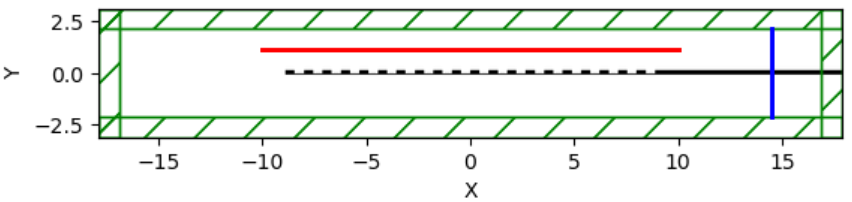
\includegraphics[width=1\linewidth]{Image/geo.png}
    \caption{Géométrie du dispositif simulé ($\mu$m)}
    \label{fig:schema_disp}
\end{figure}

Le réseau est caractérisé par sa période $\Lambda$ et son duty cycle (fraction de silicium par période). Ces deux paramètres font l'objet de l'optimisation présentée au chapitre~\ref{ch:resultats}. Le réseau se prolonge par un guide d'onde de sortie monomode, de pleine épaisseur, sur une longueur suffisante pour permettre la mesure du mode guidé loin de toute perturbation géométrique.

\section{Modélisation de la source}

La lumière incidente est modélisée par un faisceau gaussien (\texttt{GaussianBeam2DSource} sous Meep) plutôt que par une onde plane infinie, afin de représenter fidèlement le profil transverse du mode d'une fibre optique monomode standard. Le rayon au col du faisceau est fixé à $w_0=5{,}2$~\textmu m, correspondant à la moitié du diamètre de mode (MFD $\approx$10,4~\textmu m) d'une fibre SMF-28 à 1550~nm.

Le faisceau est injecté avec un angle d'incidence $\theta=10^\circ$ par rapport à la normale au guide, choix standard permettant d'éviter qu'une partie de la lumière réfléchie ne reparte directement dans la fibre par réflexion spéculaire (réflexion de Fresnel à incidence normale). Le point focal du faisceau est placé au centre du réseau, à une distance de 1~\textmu m au-dessus de la surface du guide.

L'angle d'incidence est imposé non pas en orientant physiquement la région source (nécessairement alignée sur les axes de la grille FDTD), mais via le paramètre de direction de propagation du faisceau gaussien (\texttt{beam\_kdir}), qui détermine analytiquement l'amplitude et la phase du champ le long de la ligne source pour reproduire un front d'onde incliné.

\section{Paramètres physiques des simulations}

Le tableau~\ref{tab:parametres} résume l'ensemble des paramètres fixes utilisés pour construire la géométrie et la source dans les simulations présentées dans ce rapport, indépendamment des paramètres du réseau ($\Lambda$, $gdc$) qui font l'objet de l'optimisation.

\begin{table}[h]
\centering
\begin{tabular}{lcl}
\hline
Paramètre & Valeur & Description \\
\hline
$\lambda$ & 1,55~\textmu m & longueur d'onde de conception \\
$\theta$ & $10^\circ$ & angle d'incidence de la fibre \\
$h$ & 0,22~\textmu m & épaisseur totale du slab silicium \\
$t_{slab}$ & 0,07~\textmu m & épaisseur de la base non gravée \\
$t_{etch}$ & 0,15~\textmu m & hauteur de la partie gravée ($h-t_{slab}$) \\
$N$ & 20 & nombre de dents du réseau \\
$d_{\text{PML}}$ & 1~\textmu m & épaisseur des couches absorbantes \\
$L_{wg}$ & 8~\textmu m & longueur du guide de sortie \\
$d_{\text{air}}$ & 2~\textmu m & marge d'air au-dessus/en dessous du slab \\
$w_0$ & 5,2~\textmu m & rayon au col du faisceau gaussien \\
$d_{\text{standoff}}$ & 1~\textmu m & distance source--surface du réseau \\
résolution & 150~pixels/\textmu m & résolution spatiale FDTD retenue \\
\hline
\end{tabular}
\caption{Paramètres physiques fixes utilisés dans les simulations}
\label{tab:parametres}
\end{table}


%%%%%%%%%%%%%%%%%%%%%%%%%%%%%%%%%% Chapitre 4 : Validation numerique %%%%%%%%%%%%%%%%%%%%%%%%%%%%%%%%%%
\chapter{Validation numérique}
\label{ch:validation}


Avant d'interpréter les résultats d'optimisation présentés au chapitre~\ref{ch:resultats}, il est nécessaire de s'assurer que les valeurs d'efficacité calculées reflètent bien un comportement physique et non un artefact de la discrétisation spatiale. Ce chapitre présente la démarche de validation suivie, motivée par des incohérences observées lors des premiers balayages paramétriques.

\section{Sensibilité à la discrétisation spatiale}

Meep ne discrétise pas les interfaces matériau/air de façon binaire (tout-ou-rien pixel par pixel), mais utilise une technique de moyennage sous-maille (\emph{subpixel averaging}) : lorsque le bord d'un objet géométrique tombe à l'intérieur d'un pixel plutôt que sur une frontière exacte de la grille, une permittivité effective, moyenne pondérée entre les deux matériaux, est attribuée à ce pixel. Cette approche permet en principe d'obtenir une précision supérieure à la taille d'un pixel, y compris pour des géométries mal alignées sur la grille.

Cette technique réduit l'erreur de discrétisation sans toutefois l'annuler complètement : une petite erreur résiduelle subsiste à chaque interface. Dans le cas du réseau étudié, cette erreur se répète sur les bords des $N=20$ dents, ce qui peut conduire à une accumulation significative, en particulier pour une structure à fort contraste d'indice (silicium/air, $\Delta\varepsilon=11$) où cette méthode de moyennage est réputée moins précise.

Un premier balayage paramétrique sur la période du réseau $\Lambda$ a mis en évidence ce phénomène : les valeurs d'efficacité obtenues variaient de façon non monotone et erratique avec $\Lambda$, sans forme de courbe physiquement cohérente. La cause identifiée est un défaut d'alignement entre les dimensions géométriques (période, largeur des dents, épaisseur de gravure) et la grille de calcul, chaque configuration testée retombant de façon incontrôlée sur un alignement de pixels différent.

\paragraph{Correction : alignement sur la grille (\emph{snapping}).} Pour éliminer cette source de bruit, chaque dimension géométrique a été systématiquement arrondie au multiple entier le plus proche de la taille d'un pixel ($1/\text{résolution}$) avant construction de la géométrie :
\begin{equation}
x_{\text{snap}} = \text{round}\left(\frac{x}{\Delta_{\text{pixel}}}\right)\times\Delta_{\text{pixel}}, \qquad \Delta_{\text{pixel}}=\frac{1}{\text{résolution}}
\label{eq:snap}
\end{equation}

Ce traitement a été appliqué non seulement à la période $\Lambda$, mais également à la position d'origine du réseau et à l'épaisseur de la base non gravée, afin que \emph{tous} les bords de \emph{tous} les blocs de matériau tombent exactement sur des positions de grille. Après cette correction, le balayage sur $\Lambda$ a retrouvé une forme de courbe lisse et monotone (figure~\ref{fig:balayage_lambda}), confirmant que l'irrégularité initiale était bien un artefact numérique et non un comportement physique.

\section{Étude de convergence en résolution}
\label{sec:convergence}

Une fois le bruit d'alignement éliminé, la stabilité des résultats vis-à-vis de la résolution spatiale elle-même a été vérifiée. Le point de fonctionnement ($\Lambda=0{,}72$~\textmu m, $gdc=0{,}5$) a été recalculé à résolution croissante :

\begin{table}[h]
\centering
\begin{tabular}{cc}
\hline
Résolution (pixels/\textmu m) & Efficacité (dB) \\
\hline
50  & $-12,72$ \\
100 & $-16,67$ \\
150 & $-19,29$ \\
\hline
\end{tabular}
\caption{Efficacité au point $(\Lambda,gdc)=(0{,}72,\,0{,}5)$ en fonction de la résolution}
\label{tab:convergence}
\end{table}

L'écart observé entre 50 et 100 pixels/\textmu m (environ 4~dB), puis encore entre 100 et 150 pixels/\textmu m (environ 2{,}6~dB), indique que la convergence numérique n'était pas encore pleinement atteinte, même à 100~pixels/\textmu m, ce qui est cohérent avec les dimensions sub-longueur d'onde des éléments du réseau (dents de l'ordre de 300~nm, soit seulement 15 à 45 pixels selon la résolution). La résolution de 150~pixels/\textmu m a été retenue pour l'ensemble des résultats présentés au chapitre~\ref{ch:resultats}, comme meilleur compromis atteint entre précision numérique et coût de calcul dans le temps disponible pour le projet, ce dernier croissant approximativement comme le cube de la résolution en deux dimensions (deux facteurs liés au raffinement spatial, un facteur lié à la réduction du pas de temps imposée par la condition de stabilité de Courant), sans garantie que la convergence totale soit atteinte à cette résolution.

%%%%%%%%%%%%%%%%%%%%%%%%%%%%%%%%%% Chapitre 5 : Resultats %%%%%%%%%%%%%%%%%%%%%%%%%%%%%%%%%%
\chapter{Résultats --- optimisation des paramètres}
\label{ch:resultats}

\section{Optimisation de la période du réseau}
Un balayage a été effectué manuellement pour différentes valeurs de la période, autour de l'estimation analytique initiale, afin d'identifier empiriquement la valeur optimale. Après correction des artefacts de discrétisation (alignement des dimensions géométriques sur la grille FDTD) et étude de convergence en résolution (section~\ref{sec:convergence}), une résolution de 150~pixels/\textmu m a été retenue pour ce balayage, les résultats suivants ont été obtenus :

\begin{table}[h]
\centering
\begin{tabular}{cc}
\hline
$\Lambda$ (\textmu m) & Efficacité (dB) \\
\hline
0,50 & $-37,73$ \\
0,60 & $-33,17$ \\
0,70 & $-22,86$ \\
0,72 & $-19,29$ \\
0,74 & $-16,75$ \\
0,76 & $-15,84$ \\
0,78 & $-17,52$ \\
0,80 & $-22,79$ \\
0,90 & $-44,53$ \\
\hline
\end{tabular}
\caption{Résultats du balayage sur la période du réseau, à $gdc=0{,}5$ fixe}
\label{tab:balayage_lambda}
\end{table}

La courbe obtenue présente une forme en cloche nette autour de $\Lambda=0{,}76$~\textmu m (figure~\ref{fig:balayage_lambda}), avec une décroissance rapide de part et d'autre de ce sommet. Cette valeur diffère légèrement de l'optimum identifié à résolution plus faible (100~pixels/\textmu m, $\Lambda=0{,}72$~\textmu m), ce qui confirme que la convergence numérique n'était pas encore pleinement atteinte à cette résolution intermédiaire.

La période optimale ainsi déterminée, $\Lambda_{opt}=0{,}76$~\textmu m, sera utilisée comme référence pour l'exploration du duty cycle ci-après et comme point de départ pour l'optimisation par gradient présentée en section~\ref{sec:adjoint}.

\begin{figure}[h]
    \centering
    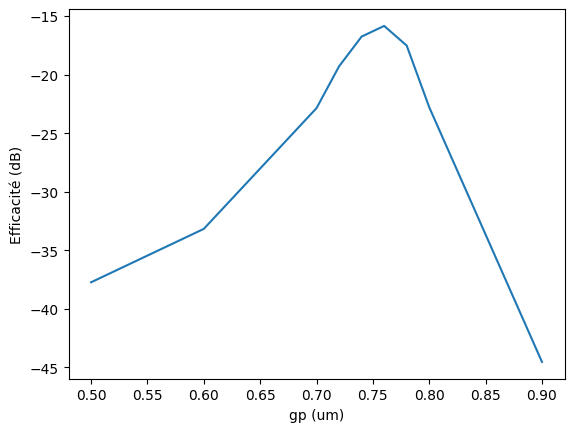
\includegraphics[width=0.7\linewidth]{Image/gp_r150.png}
    \caption{Résultats du balayage des valeurs de la période, à résolution 150~pixels/\textmu m avec le duty cycle fixé à 0{,}5}
    \label{fig:balayage_lambda}
\end{figure}


\vspace{0.5em}

\section{Exploration du duty cycle et limites de l'étude}
\label{sec:duty_cycle}

Un balayage similaire a été effectué pour le duty cycle (proportion de silicium par période), à période fixée $\Lambda=0{,}72$~\textmu m et à résolution 150~pixels/\textmu m. Les résultats suivants ont été obtenus :

\subsection*{Tests sur les valeurs du duty cycle}
\begin{table}[h]
\centering
\begin{tabular}{cc}
\hline
$gdc$ & Efficacité (dB) \\
\hline
0,40 & $-33,06$ \\
0,50 & $-19,29$ \\
0,60 & $-18,25$ \\
0,65 & $-15,76$ \\
0,67 & $-14,55$ \\
0,69 & $-13,74$ \\
0,70 & $-14,00$ \\
0,71 & $-14,64$ \\
0,73 & $-17,28$ \\
0,75 & $-22,14$ \\
0,80 & $-36,46$ \\
\hline
\end{tabular}
\caption{Résultats du balayage sur le duty cycle, à $\Lambda=0{,}72$~\textmu m fixe}
\label{tab:balayage_gdc}
\end{table}

\begin{figure}[h]
    \centering
    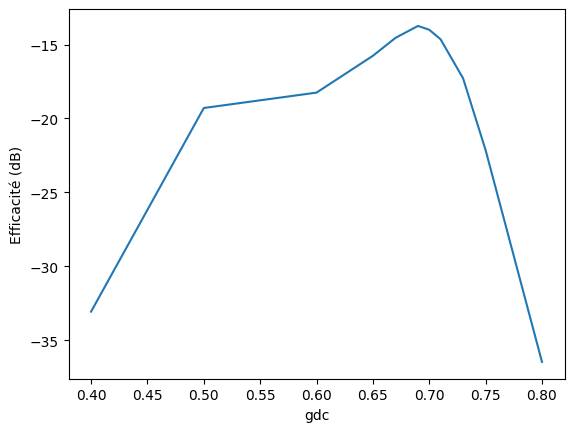
\includegraphics[width=0.7\linewidth]{Image/gdc_r150.png}
    \caption{Résultats du balayage des valeurs du duty cycle, à résolution 150~pixels/\textmu m}
    \label{fig:balayage_gdc}
\end{figure}

La courbe obtenue (figure~\ref{fig:balayage_gdc}) présente une forme en cloche resserrée, avec un maximum net à $gdc=0{,}69$ ($-13{,}74$~dB) et une décroissance rapide de part et d'autre, notamment au-delà de $gdc=0{,}73$, où l'efficacité chute de plus de 20~dB en l'espace de quelques centièmes.

\paragraph{Limite observée.} Ce second balayage, mené à $\Lambda=0{,}72$~\textmu m fixe, donne un optimum ($-13{,}74$~dB à $gdc=0{,}69$) meilleur que celui obtenu lors du balayage sur $\Lambda$ à $gdc=0{,}5$ fixe ($-19{,}29$~dB au même point $\Lambda=0{,}72$, section précédente). Cette différence confirme que l'optimum global du dispositif ne se situe pas sur les valeurs trouvées indépendamment par chacun des deux balayages séquentiels, mais dans une combinaison des deux. Cela motive le recours à une optimisation conjointe des deux paramètres par la méthode du gradient, présentée en section~\ref{sec:adjoint}.


\section{Optimisation par montée de gradient}
\label{sec:adjoint}

Une méthode d'optimisation par gradient a été mise en œuvre, en s'appuyant sur le solveur adjoint intégré à Meep pour calculer le gradient de l'efficacité de couplage par rapport aux deux paramètres du réseau ($\Lambda$, $gdc$) simultanément. Pour cette étape, la source gaussienne inclinée a été temporairement remplacée par une source classique plus simple (onde plane sans angle), le solveur adjoint s'étant révélé incompatible avec le type de source utilisé pour les résultats précédents. Les valeurs d'efficacité rapportées dans cette section ne sont donc pas directement comparables en valeur absolue à celles du balayage manuel ; l'efficacité avec la source réelle sera recalculée séparément, une fois l'optimum trouvé.

\subsection*{Point de départ proche de l'optimum manuel}

Pour cette optimisation, le solveur adjoint de Meep s'est révélé incompatible avec le type de source utilisé pour les résultats précédents (\texttt{GaussianBeam2DSource}), le calcul du gradient provoquait une erreur interne, liée à l'implémentation de cette source dans le mécanisme adjoint. La source a donc été remplacée par une onde plane simple, à laquelle l'angle d'incidence $\theta=10^\circ$ a été réintroduit via une fonction de phase (\texttt{amp\_func}) reproduisant le déphasage d'un front d'onde incliné le long de la ligne source. Cette source conserve la bonne condition d'accord de phase, mais ne reproduit pas le profil transverse gaussien du faisceau réel. 

Un essai, parti des conditions initiales $(\Lambda,gdc)=(0{,}7435,\ 0{,}6717)$, une zone déjà identifiée comme favorable par le balayage manuel, donne les résultats suivants :

\begin{table}[h]
\centering
\begin{tabular}{lcccc}
\hline
Itération & $\Lambda$ (\textmu m) & $gdc$ & Efficacité (dB) \\
\hline
1 & 0,7435 & 0,6717 & $-18,09$ \\
2 & 0,7525 & 0,6834 & $-16,78$ \\
3 & 0,7612 & 0,6856 & $-15,65$ \\
4 & 0,7590 & 0,6823 & $-10,55$ \\
5 & 0,7596 & 0,6819 & $-10,36$ \\
6 & 0,7652 & 0,6836 & $-12,10$ \\
\hline
\end{tabular}
\caption{Itérations de l'optimisation par gradient (onde plane inclinée à $10^\circ$, angle réintroduit via une fonction de phase)}
\label{tab:gradient_iterations}
\end{table}

Malgré une oscillation résiduelle, l'algorithme progresse de façon cohérente avec l'optimum du balayage manuel ($gdc\approx0{,}69$, section~\ref{sec:duty_cycle}), atteignant $-10{,}36$~dB à l'itération 5 avec cette source simplifiée, une amélioration de près de 8~dB par rapport au point de départ.

\paragraph{Calcul final avec la source réelle.} Les valeurs d'efficacité ci-dessus, obtenues avec l'onde plane inclinée, ne sont pas directement comparables à celles du balayage manuel (mesurées avec le vrai faisceau gaussien). Le meilleur point trouvé par le gradient ($\Lambda=0{,}7596$~\textmu m, $gdc=0{,}6819$) a donc été recalculé avec la source gaussienne réelle ($w_0=5{,}2$~\textmu m, $\theta=10^\circ$), sur la géométrie utilisée par l'optimisation adjointe. Ce calcul donne une efficacité de $-13{,}39$~dB, une valeur inférieure au $-10{,}36$~dB obtenu avec l'onde plane, mais qui reste toutefois cohérent avec l'optimum du balayage manuel ($-13{,}74$~dB). Cet écart confirme que l'onde plane inclinée, bien qu'elle restaure correctement la condition d'accord de phase, ne reproduit pas la même physique de couplage qu'un faisceau gaussien réel : l'optimum trouvé pour un éclairage uniforme du réseau ne correspond pas exactement à l'optimum pour un faisceau localisé, dont le recouvrement avec le profil de rayonnement du réseau dépend de paramètres non pris en compte ici.

\section{Comparaison des modèles analytiques et numériques}

Le tableau~\ref{tab:comparaison_finale} synthétise les prédictions des différents modèles développés au chapitre~\ref{ch:theorie}, confrontées aux résultats numériques obtenus par balayage manuel puis par optimisation par gradient.

\begin{table}[h]
\centering
\begin{tabular}{lccc}
\hline
Méthode & $\Lambda$ (nm) & $gdc$ & Efficacité (dB) \\
\hline
Pondération volumique (analytique) & 762 & 0,50 (fixé) & --- \\
Modèle multicouche (analytique) & 758 & 0,50 (fixé) & --- \\
Balayage manuel (FDTD, source réelle) & 720 & 0,69 (optimisé) & $-13,74$ \\
Optimisation par gradient (FDTD, source réelle) & 759,6 & 0,6819 (optimisé) & $-13,39$ \\
\hline
\end{tabular}
\caption{Comparaison des périodes prédites par les modèles analytiques et des résultats numériques}
\label{tab:comparaison_finale}
\end{table}

Les deux modèles analytiques, évalués à $gdc=0{,}5$ (une valeur fixée en entrée, non optimisée par ces modèles), prédisent une période très proche de l'optimum FDTD, confirmant qu'une bonne partie de la physique de l'accord de phase est déjà capturée sans simulation FDTD complète. Cette comparaison ne concerne toutefois que la période : ces modèles analytiques ne fournissent aucune indication sur la valeur optimale du duty cycle lui-même, seul le balayage FDTD et l'optimisation par gradient ayant permis de l'identifier.

L'optimisation par gradient, une fois son résultat recalculé avec la source Gaussienne, converge vers une efficacité ($-13{,}39$~dB) très proche de celle du balayage manuel ($-13{,}74$~dB), sur un point légèrement différent ($\Lambda=759{,}6$~nm, $gdc=0{,}6819$ contre $720$~nm, $0{,}69$). 

\section{Ajout d'un réflecteur inférieur}

\subsection*{Position du problème}

Dans la géométrie étudiée jusqu'ici, le milieu sous le réseau est symétrique à la gaine supérieure (air), la moitié de la puissance diffractée vers le bas est donc perdue. On décide ainsi d'étudier l'ajout d'une couche d'oxyde enterré (BOX, \textit{Buried OXide}, d'indice $n_{BOX}\approx1{,}44$) entre le silicium et le substrat, dont l'épaisseur $t_{BOX}$ est choisie pour renvoyer cette lumière vers le haut par interférence constructive, plutôt que de la laisser se transmettre dans le substrat.
On a donc le schéma suivant :
\begin{figure}[H]
    \centering
    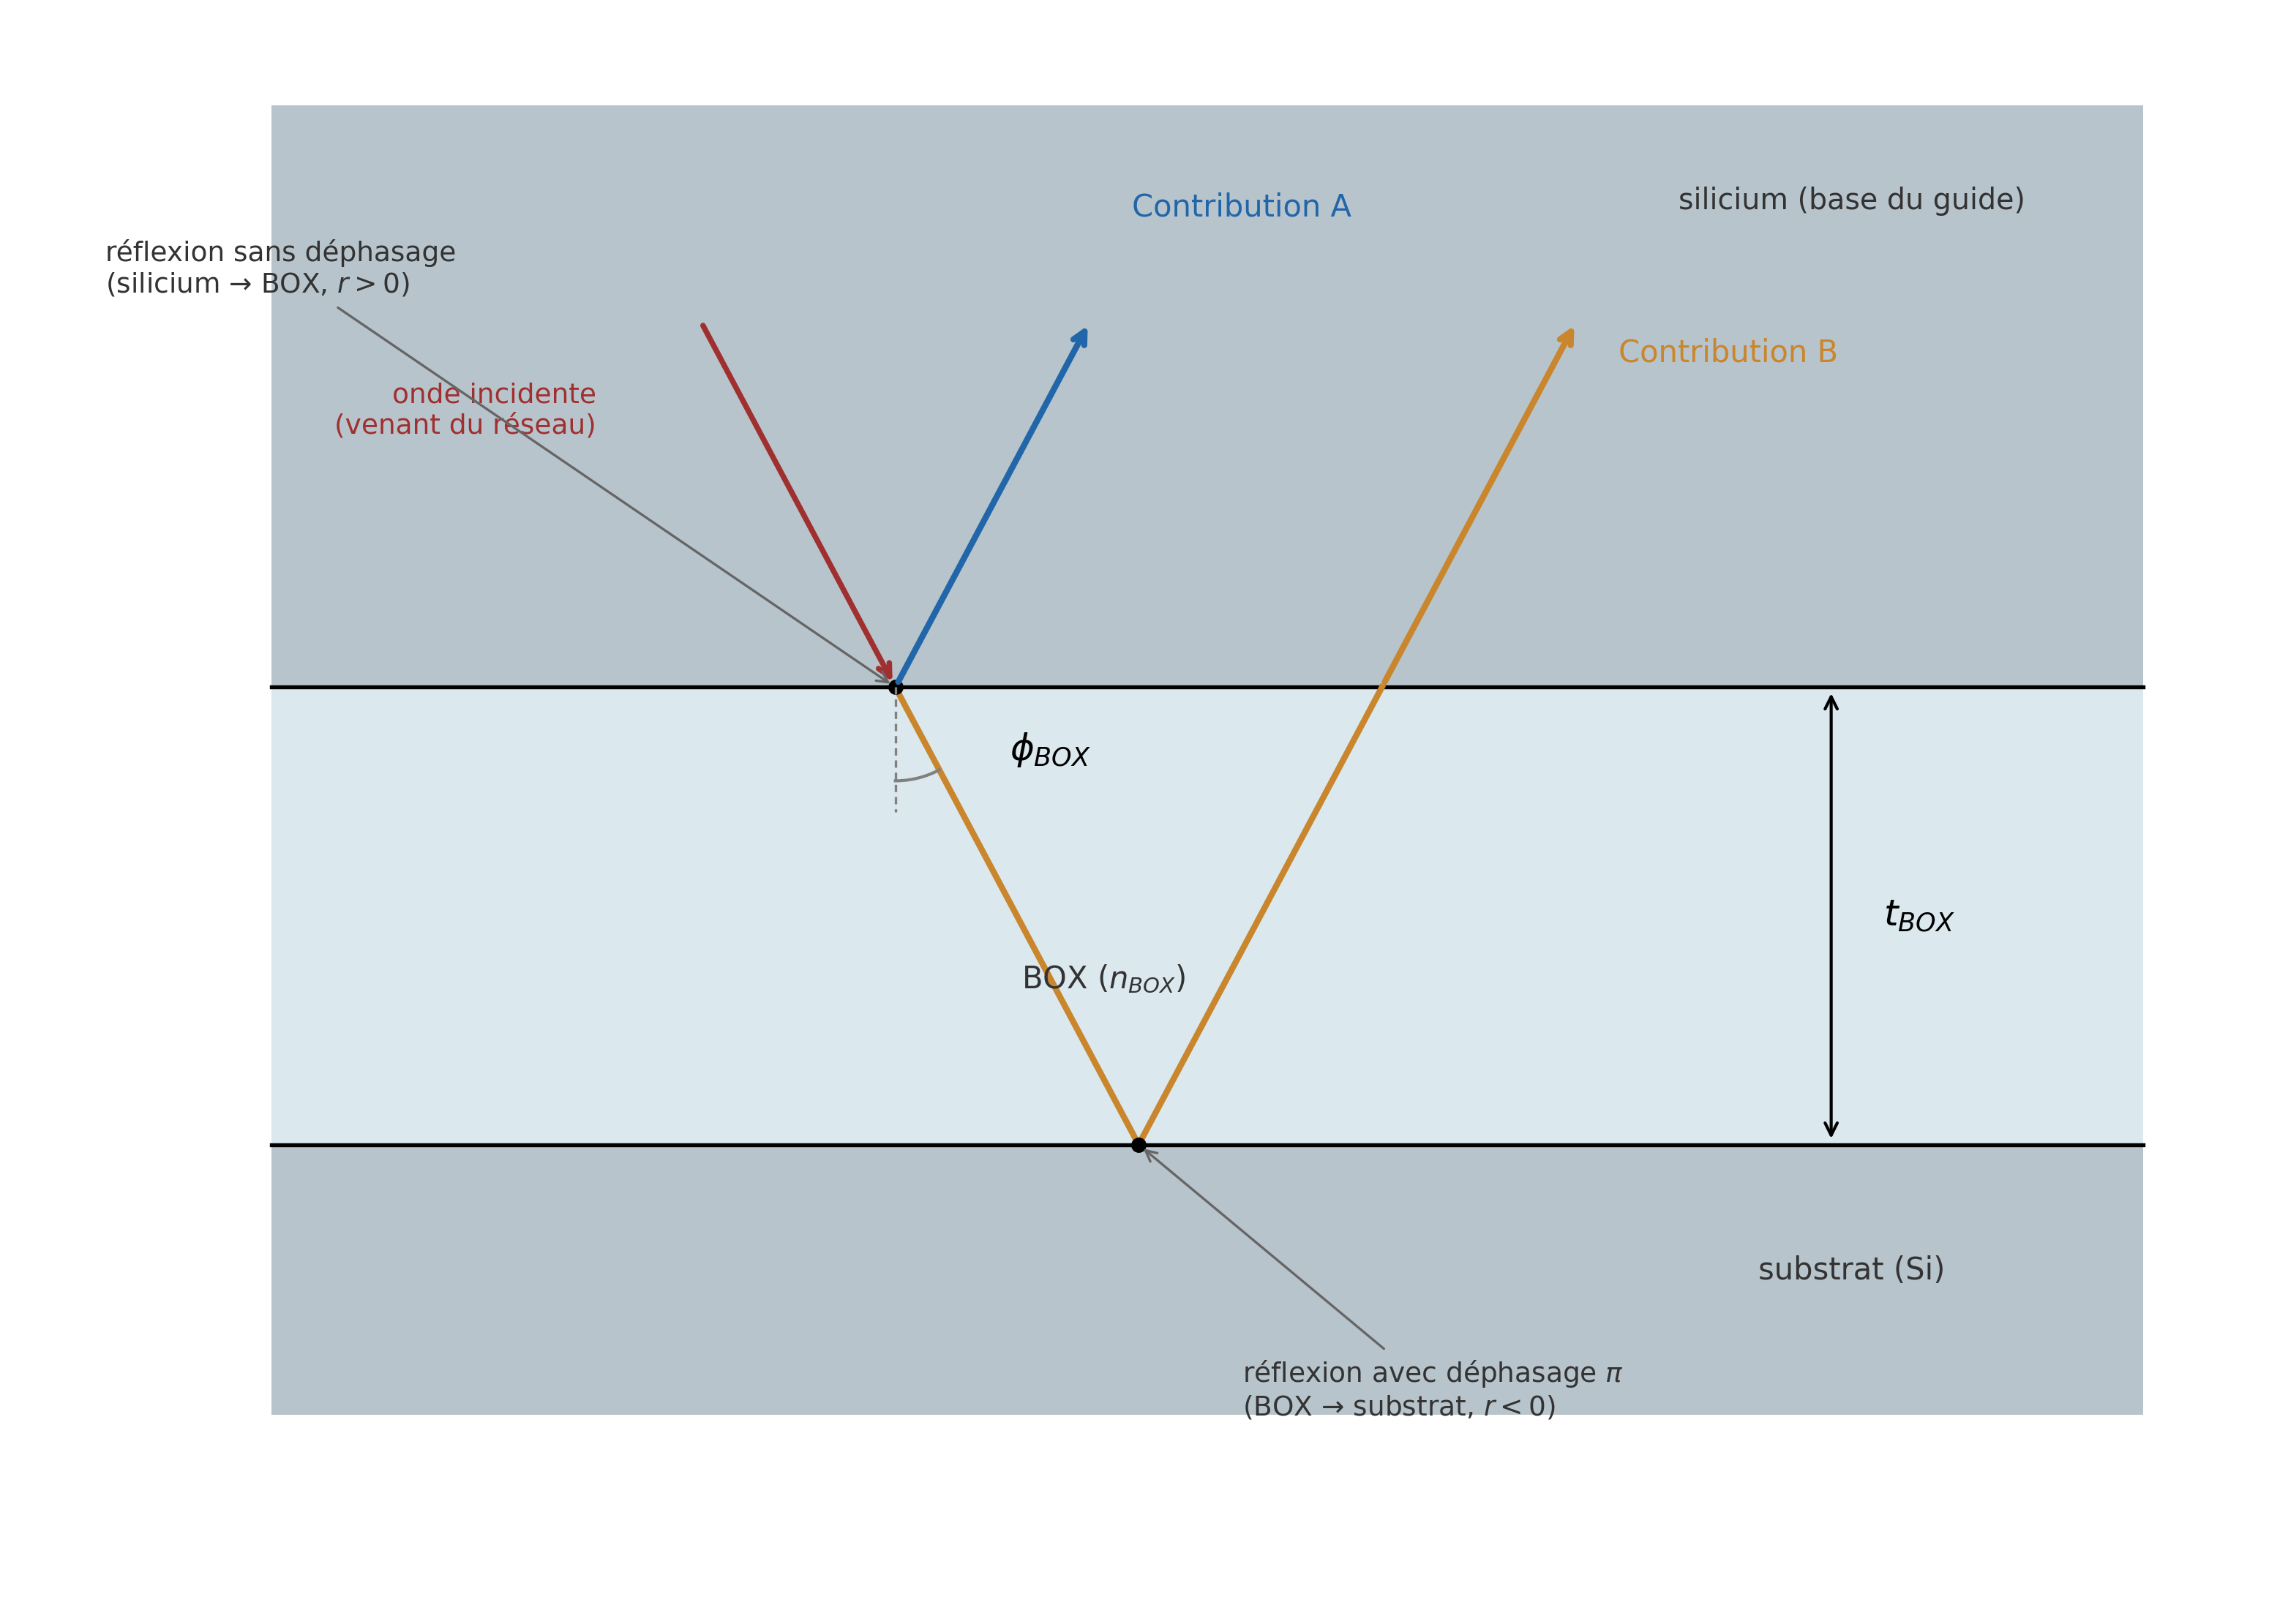
\includegraphics[width=1\linewidth]{Image/schema_box_diff_marche.png}
    \caption{Trajets des contributions A et B pour le calcul de la différence de marche dans le réflecteur BOX}
    \label{fig:box_diff_marche}
\end{figure}
\begin{itemize}
    \item \textbf{Contribution A} : réflexion directe à la première interface (silicium~$\rightarrow$~BOX) ;
    \item \textbf{Contribution B} : transmission dans le BOX, réflexion à la seconde interface (BOX~$\rightarrow$~substrat), puis retour à travers le BOX.
\end{itemize}

\subsection*{Déphasage à la réflexion}

D'après les équations de Fresnel à incidence normale, le coefficient de réflexion à une interface entre un milieu d'indice $n_1$ (incident) et un milieu d'indice $n_2$ (transmis) s'écrit $r=(n_1-n_2)/(n_1+n_2)$. Son signe déterminera un déphasage de $0$ ou $\pi$ :

\begin{itemize}
    \item \textbf{Interface silicium~$\rightarrow$~BOX} ($n_1=n_{Si}>n_2=n_{BOX}$) : $r_1>0$, pas de déphasage supplémentaire à la réflexion (contribution A) ;
    \item \textbf{Interface BOX~$\rightarrow$~substrat} ($n_1=n_{BOX}<n_2=n_{Si}$) : $r_2<0$, ce qui correspond à un déphasage supplémentaire de $\pi$ à la réflexion (contribution B).
\end{itemize}

\subsection*{Différence de marche et condition d'interférence constructive}

La lumière diffractée par le réseau atteint le BOX avec un angle $\phi_{BOX}$ par rapport à la normale. La contribution B parcourt, par rapport à la contribution A, une distance optique supplémentaire correspondant à l'aller-retour dans la couche de BOX. On a donc l'expression suivante :
\begin{equation}
\delta_{BOX} = \frac{2\,n_{BOX}\,t_{BOX}}{\cos\phi_{BOX}}
\end{equation}
On obtient ainsi un déphasage égal à :
\begin{equation}
\Delta\varphi = \dfrac{2\pi}{\lambda}\,\delta_{BOX} = \dfrac{4\pi\,n_{BOX}\,t_{BOX}}{\lambda\cos\phi_{BOX}}
\end{equation}
En tenant compte du déphasage supplémentaire de $\pi$ subi par la contribution B à sa réflexion (et non par la contribution A), le déphasage total entre les deux contributions est :
\begin{equation}
\Delta\varphi = \frac{4\pi\,n_{BOX}\,t_{BOX}}{\lambda\cos\phi_{BOX}} + \pi
\end{equation}
Pour que les deux contributions interfèrent de façon constructive, il faut que ce déphasage soit un multiple entier de 2$\pi$ :
\begin{equation}
\Delta\varphi = 2m\pi, \qquad m\in\mathbb{N}^*
\end{equation}
On a donc :
\begin{equation}
\frac{4\pi\,n_{BOX}\,t_{BOX}}{\lambda\cos\phi_{BOX}} = (2m-1)\pi
\end{equation}
On a ainsi :
\begin{equation}
\boxed{t_{BOX} = \frac{(2m-1)\,\lambda\,\cos\phi_{BOX}}{4\,n_{BOX}}}
\label{eq:box_quarter_wave}
\end{equation}

\subsection*{Résultat numérique}

Avec $\lambda=1{,}55$~\textmu m et $n_{BOX}=1{,}44$ (et un angle d'incidence nulle), les premières épaisseurs candidates sont :
\begin{equation}
t_{BOX}\approx0{,}269~\text{\textmu m}\ (m=1), \quad 0{,}807~\text{\textmu m}\ (m=2), \quad 1{,}345~\text{\textmu m}\ (m=3)
\end{equation}
Ces valeurs servent de point de départ à un balayage FDTD, la géométrie et le réseau ($\Lambda$, $gdc$) restant fixés à l'optimum déterminé précédemment.

\paragraph{Résultat.}Le balayage effectué (épaisseurs de 0{,}03 à 1{,}0~\textmu m) n'a pas permis d'identifier d'épaisseur de BOX améliorant l'efficacité par rapport à la géométrie sans réflecteur ($-13{,}39$~dB). Toutes les valeurs testées donnent un résultat inférieur, avec un maximum local à $-15{,}97$~dB pour $t_{BOX}=0{,}06$~\textmu m. Ce résultat suggère que le modèle simplifié à deux ondes (interférence entre les deux premières réflexions) utilisé pour l'estimation analytique est insuffisant. La couche mince intercalée entre deux milieux de silicium semble en fait former une cavité de Fabry-Pérot à réflexions multiples, dont le comportement est difficile à prévoir. Une étude théorique plus poussée serait nécessaire pour conclure sur le potentiel de ce réflecteur, cela n'a cependant pas pu être effectué dans le temps imparti. 

Le tableau~\ref{tab:box_balayage} présente les résultats du balayage sur l'épaisseur du BOX, à $\Lambda$ et $gdc$ fixés à l'optimum précédemment déterminé.
\begin{table}[h]
\centering
\begin{tabular}{cc}
\hline
$t_{BOX}$ (\textmu m) & Efficacité (dB) \\
\hline
--- (sans BOX, référence) & $-13,39$ \\
0,030 & $-25,93$ \\
0,060 & $-15,97$ \\
0,090 & $-17,33$ \\
0,120 & $-19,63$ \\
0,150 & $-20,80$ \\
0,200 & $-26,24$ \\
0,270 & $-33,52$ \\
0,350 & $-31,46$ \\
0,450 & $-30,07$ \\
0,600 & $-23,13$ \\
0,807 & $-37,01$ \\
1,000 & $-25,28$ \\
\hline
\end{tabular}
\caption{Résultats du balayage sur l'épaisseur du réflecteur BOX, à $\Lambda$ et $gdc$ fixés à l'optimum}
\label{tab:box_balayage}
\end{table}

\chapter{Conclusion}

\section{Bilan}

Ce projet visait à concevoir, simuler et optimiser un coupleur à réseau fibre-puce en silicium, en combinant une approche analytique et une simulation FDTD sous Meep. La démarche a suivi un déroulement cohérent : une estimation théorique initiale de la période du réseau, affinée progressivement par des modèles analytiques de plus en plus fidèles à la géométrie réelle (pondération volumique, puis modèle multicouche par matrices de transfert) ; une mise en œuvre numérique rigoureuse, validée par une étude de la sensibilité à la discrétisation spatiale et de la convergence en résolution ; puis une optimisation des paramètres du réseau, menée à la fois par balayage paramétrique manuel et par une méthode de gradient s'appuyant sur le solveur adjoint de Meep.

Les deux modèles analytiques les plus aboutis prédisent une période de $758$ à $762$~nm, très proche de l'optimum identifié numériquement ($760$~nm), confirmant qu'une part importante de la physique du couplage (condition d'interférence constructive) est correctement capturée par un modèle simplifié de l'indice effectif, sans nécessiter de simulation complète. L'optimisation des deux paramètres du réseau ($\Lambda$, $gdc$), menée par balayage manuel puis par gradient, a permis d'atteindre une efficacité de couplage de $-13{,}4$~dB (environ $4{,}6\%$), les deux méthodes convergeant vers des points très voisins de l'espace des paramètres.

\section{Limites de l'étude}

Plusieurs limites ont été identifiées au cours du projet, expliquant l'écart entre l'efficacité obtenue et les valeurs typiquement vues dans les publications sur ce type de composants (typiquement $-1$ à $-3$~dB) :

\begin{itemize}
    \item \textbf{Absence de réflecteur inférieur efficace.} L'ajout d'une couche d'oxyde enterré (BOX), censé rediriger vers la fibre la moitié de la puissance diffractée vers le substrat, n'a pas permis d'amélioration dans le balayage effectué. Ce résultat s'explique par la limite du modèle analytique utilisé, une approximation à deux ondes, alors que la structure forme en réalité une cavité de Fabry-Pérot à réflexions bien plus nombreuses et complexes.
    \item \textbf{Réseau uniforme, non apodisé.} Même dans le cas idéal, un réseau à dents identiques ne peut pas parfaitement correspondre au profil gaussien du faisceau incident, ce qui diminue donc l'efficacité finale mesurée.
    \item \textbf{Optimisation partiellement conjointe.} Seuls deux paramètres géométriques ($\Lambda$, $gdc$) ont été optimisés, parmi les cinq ou six qui influencent réellement l'efficacité (profondeur de gravure, position du point focal, nombre de dents, épaisseur du BOX).
    \item \textbf{Source Gaussienne incompatible avec l'optimisation par gradient} Le solveur adjoint de Meep s'est révélé incompatible avec la source en faisceau gaussien utilisée pour les résultats de référence. La source a dû être simplifiée (onde plane, puis onde plane inclinée par une fonction de phase) pour cette étape, avec un recalcul final nécessaire pour obtenir un résultat comparable aux autres méthodes.
    \item \textbf{Modélisation bidimensionnelle.} L'ensemble de l'étude repose sur une approximation 2D, qui ignore le confinement latéral réel d'un guide de largeur finie et les pertes associées.
\end{itemize}

\section{Perspectives}

Plusieurs pistes, identifiées mais non explorées dans le temps imparti à ce projet, permettraient d'améliorer significativement l'efficacité obtenue :

\begin{itemize}
    \item faire varier la profondeur de gravure et le duty cycle le long du réseau (apodisation) pour mieux correspondre au profil gaussien du faisceau incident ;
    \item une modélisation plus rigoureuse du réflecteur BOX, prenant en compte les réflexions multiples ;
    \item une meilleure optimisation par gradient adjoint, qui permettrait d'explorer des géométries de réseau plus complexes.
\end{itemize}
\end{document}
